\documentclass[hidelinks]{article}
\usepackage[letterpaper,margin=1.0in]{geometry}
\usepackage[utf8]{inputenc}
\pagenumbering{arabic}
\usepackage{authblk}
\usepackage{graphicx}
\usepackage[singlelinecheck=false]{caption} % singlelinecheck makes single line caption left aligned instead of centered
\usepackage{subcaption}
\usepackage{amsmath}
\usepackage[round]{natbib}
\usepackage{fancyhdr}
\usepackage{longtable}
\usepackage{booktabs}
% hyperlinks
\usepackage{hyperref}
\usepackage{wrapfig}
\usepackage{xspace}
\usepackage{mathrsfs}
\usepackage{graphicx}
\usepackage{lipsum}

\pagestyle{fancy}
\fancyhead[R]{\textbf{Expanding \stdpopsim}}

% for highlighting text
\usepackage{xcolor}
\usepackage{soul}

% bibliography
\usepackage[round]{natbib}   % omit 'round' option if you prefer square brackets
\bibliographystyle{plainnat}



\newcommand{\Stdpopsim}{\texttt{Stdpopsim}\xspace}
\newcommand{\stdpopsim}{\texttt{stdpopsim}\xspace}

%commands to format figure and table references in the supplement
\newcommand{\beginsupplement}{%
        \fancyhead[L]{Supplemental Material}
        \setcounter{table}{0}
        \renewcommand{\thetable}{S\arabic{table}}%
        \setcounter{figure}{0}
        \renewcommand{\thefigure}{S\arabic{figure}}%
     }
\newcommand{\stopsupplement}{%
        \setcounter{table}{0}
        \renewcommand{\thetable}{\arabic{table}}%
        \setcounter{figure}{0}
        \renewcommand{\thefigure}{\arabic{figure}}%
     }

\makeatletter
\newcommand{\labelname}[1]{\def\@currentlabelname{#1}}
\makeatother

% Avoid pandoc bug when there are lists in the body.
\providecommand{\tightlist}{%
\setlength{\itemsep}{0pt}\setlength{\parskip}{0pt}}

\title{Adding selection to \stdpopsim: oh how the tables have turned}


% \author[1,+]{M. Elise Lauterbur}
% \author[3,*]{Ariella L. Gladstein}
 \author[4,*]{Graham Gower}
 \author[5*]{Nathaniel S. Pope}
 \author[5*]{Murillo F. Rodrigues}
\author[6]{Georgia Tsambos}
\author[34]{Linh N. Tran}
\author[2]{Maria Izabel A. Cavassim}
% \author[5,7]{Jeff Adrion}
% \author[5]{Saurabh Belsare}
% \author[8]{Arjun Biddanda}
% \author[5]{Victoria Caudill}
% \author[9]{Jean Cury}
% \author[10]{Ignacio Echevarria}
% \author[11]{Benjamin C. Haller}
% \author[12,13]{Ahmed R. Hasan}
\author[14,15]{Xin Huang}
% \author[16]{Leonardo Nicola Martin Iasi}
% \author[17]{Ekaterina Noskova}
% \author[18]{Jana Obšteter}
% \author[19]{Vitor Antonio Corrêa Pavinato}
% \author[20,21]{Alice Pearson}
% \author[22,23]{David Peede}
% \author[24]{Manolo F. Perez}
\author[5]{Chris C. R. Smith}
% \author[25]{Jeffrey P. Spence}
% \author[5]{Anastasia Teterina}
\author[5]{Silas Tittes}
\author[5]{Scott T. Small}
% \author[26]{Per Unneberg}
% \author[27]{Juan Manuel Vazquez}
% \author[28]{Ryan K. Waples}
% \author[29]{Anthony Wilder Wohns}
% \author[30]{Yan Wong}
% \author[31]{Franz Baumdicker}
% \author[32]{Reed A. Cartwright}
% \author[33]{Gregor Gorjanc}
\author[4]{Kirk E. Lohmueller}
\author[34]{Ryan N. Gutenkunst}
\author[30]{Jerome Kelleher}
\author[35]{Aaron P. Ragsdale}

\author[37]{Daniel R. Schrider}
\author[38]{Ilan Gronau}
\author[5,36]{Peter L. Ralph}
\author[5]{Andrew D. Kern}


 \affil[*]{\small{These authors contributed equally to the paper.}}
% \affil[+]{\small{Corresponding authors: lauterbur@gmail.com ; ilan.gronau@runi.ac.il.}}
% \affil[1]{\small{Department of Ecology and Evolutionary Biology, University of Arizona, Tucson AZ 85719, USA}}
% \affil[2]{\small{Department of Ecology and Evolutionary Biology, University of California, Los Angeles, Los Angeles CA, USA}}
% \affil[3]{\small{Embark Veterinary, Inc., Boston MA 02111, USA}}
 \affil[4]{\small{Section for Molecular Ecology and Evolution, Globe Institute, University of Copenhagen, Denmark}}
 \affil[5]{\small{Institute of Ecology and Evolution, University of Oregon, Eugene OR 97402, USA}}
% \affil[6]{\small{School of Mathematics and Statistics, University of Melbourne, Australia}}
% \affil[7]{\small{AncestryDNA, San Francisco CA 94107, USA}}
% \affil[8]{\small{54Gene, Inc., Washington DC 20005, USA}}
% \affil[9]{\small{Université Paris-Saclay, CNRS, INRIA, Laboratoire Interdisciplinaire des Sciences du Numérique, UMR 9015 Orsay, France}}
% \affil[10]{\small{School of Life Sciences, University of Glasgow, Glasgow, UK}}
% \affil[11]{\small{Department of Computational Biology, Cornell University, Ithaca NY, USA}}
% \affil[12]{\small{Department of Cell and Systems Biology, University of Toronto, Toronto ON, Canada}}
% \affil[13]{\small{Department of Biology, University of Toronto Mississauga, Mississauga ON, Canada}}
% \affil[14]{\small{Department of Evolutionary Anthropology, University of Vienna, Vienna, Austria}}
% \affil[15]{\small{Human Evolution and Archaeological Sciences (HEAS), University of Vienna, Vienna, Austria}}
% \affil[16]{\small{Department of Evolutionary Genetics, Max Planck Institute for Evolutionary Anthropology, Leipzig, Germany}}
% \affil[17]{\small{Computer Technologies Laboratory, ITMO University, St Petersburg, Russia}}
% \affil[18]{\small{Agricultural Institute of Slovenia, Department of Animal Science, Ljubljana, Slovenia}}
% \affil[19]{\small{Entomology Department, The Ohio State University, Wooster OH, USA}}
% \affil[20]{\small{Department of Genetics, University of Cambridge, Cambridge, UK}}
% \affil[21]{\small{Department of Zoology, University of Cambridge, Cambridge, UK}}
% \affil[22]{\small{Department of Ecology, Evolution, and Organismal Biology, Brown University, Providence RI, USA}}
% \affil[23]{\small{Center for Computational Molecular Biology, Brown University, Providence RI, USA}}
% \affil[24]{\small{Department of Genetics and Evolution, Federal University of Sao Carlos, Sao Carlos 13565905, Brazil}}
% \affil[25]{\small{Department of Genetics, Stanford University School of Medicine, Stanford CA 94305, USA}}
% \affil[26]{\small{Department of Cell and Molecular Biology, National Bioinformatics Infrastructure Sweden, Science for Life Laboratory, Uppsala University, Husargatan 3, SE-752 37 Uppsala, Sweden}}
% \affil[27]{\small{Department of Integrative Biology, University of California, Berkeley, Berkeley CA, USA}}
% \affil[28]{\small{Department of Biostatistics, University of Washington, Seattle WA, USA}}
% \affil[29]{\small{Broad Institute of MIT and Harvard, Cambridge MA 02142, USA}}
\affil[30]{\small{Big Data Institute, Li Ka Shing Centre for Health Information and Discovery, University of Oxford, Oxford OX3 7LF, UK}}
% \affil[31]{\small{Cluster of Excellence - Controlling Microbes to Fight Infections, Eberhard Karls Universität Tübingen, Tübingen, Baden-Württemberg, Germany}}
% \affil[32]{\small{School of Life Sciences and The Biodesign Institute, Arizona State University, Tempe AZ, USA}}
% \affil[33]{\small{The Roslin Institute and Royal (Dick) School of Veterinary Studies, University of Edinburgh, Edinburgh EH25 9RG, UK}}
% \affil[34]{\small{Department of Molecular and Cellular Biology, University of Arizona, Tucson AZ 85721, USA}}
\affil[35]{\small{Department of Integrative Biology, University of Wisconsin-Madison, Madison WI, USA}}
\affil[36]{\small{Department of Mathematics, University of Oregon, Eugene OR 97402, USA}}
\affil[37]{\small{Department of Genetics, University of North Carolina at Chapel Hill, Chapel Hill NC 27599, USA}}
\affil[38]{\small{Efi Arazi School of Computer Science, Reichman University, Herzliya, Israel}}

\date{\small{\today{}}}

\begin{document}

\maketitle


\section*{Abstract}

\section*{Introduction}
    \label{introduction}
    % natural selection
    Natural selection is a fundamental force in evolution, shaping the
    genetic diversity of populations and driving the adaptation of
    species to their environments. The effects of natural selection
    on genetic variation are complex, and can be difficult to disentangle
    from other evolutionary processes such as mutation, recombination,
    and genetic drift \cite[e.g.,][]{gillespie1991causes}.
    For instance changes in population size can lead to fluctuations
    in genetic diversity across a recombining chromosome 
    that can mimic the effects of selection \citep{simonsen1995properties, barton1998effect},
    and lead to spurious inferences about the strength and targets of genetic adaptation
    \cite{simonsen1995properties,akey2004population,nielsen2005genomic}.
    In turn selection can confound our ability to infer demographic 
    history from allele frequencies \citep{ewing2016consequences} and
    estimates of inverse coalescent rate \citep{schrider2016effects}.
    Thus it is imperative to joingly account for the effects of selection
    and demography when inferring evolutionary history from genetic data
    however this is a challenging task from a modeling perspective.

    % simulation
    To meet this need the field of population genetics
    has turned to simulation.
    Simulation has become a critical tool for interpretation, 
    analysis, and exploration of realistic evolutionary models.
    Simulation in population genetics has a long history 
    including both backward in time coalescent simulations
    \citep{kingman1982genealogy,hudson1983testing, hudson1990gene}
    and forward in time simulations of complex demography and selection
    \citep[e.g.,][]{gillespie1984molecular,thornton2014c++, haller2019slim}.
    The development of simulation tools has been driven by the need to
    understand the effects of complex evolutionary processes on genetic
    variation \citep[e.g.,][]{galloway2020few}, to provide a null model for hypothesis testing
    \citep[e.g.,][]{hudson1992statistical}, to
    to explore the power and limitations of statistical methods \cite[e.g.,]{przeworski2002signature},
    and increasingly to provide a basis for machine learning and other
    simulation-based inference methods \citep[e.g.,]{kern2018diplos}.
    While this is so, joint simulation of complex demography and selection
    is challenging, and requires a deep understanding of the underlying
    evolutionary processes, as well as a number of parameter choices including
    the strength of selection, the distribution of fitness effects, and the
    recombination rate, as well as a parameterized model of demography.
    This is dounting task for many researchers, and can be a barrier to
    the adoption of simulation-based methods in population genetics.
    Further, sharing and comparing simulation results among studies can 
    itself be challenging, as different simulation tools may use different
    models and parameterizations, and may not be directly comparable.
    This is a major limitation for the field, as it can make it difficult
    to assess the robustness of results, and to compare the results of
    different studies.

    % stdpopsim
    A lingering challenge with simulation in population genetics has been
    reproducibility and the ability to share and compare results among 
    researchers \citep[][e.g.,]{ragsdale2020lessons}.
    This challenge has been addressed in part by the development
    of community resources for sharing and distributing simulation software
    via the \stdpopsim project \citep{adrion2020community}. \stdpopsim
    provides a standardized interface for accessing a wide range of
    population genetic models, and has begun to be be widely adopted by the community. %maybe add citations here?
    While that is so, the current version of \stdpopsim does not include
    models of selection, which is a major limitation for more empirical
    applications of population genetic simulation. In particular, modeling selection
    through simulation is critical for understanding the processes such
    as adaptation, the effects of selective sweeps, and the impact of
    background selection on genetic diversity. Ideally, one would like
    to have a single, unified framework for simulating both neutral and
    non-neutral evolutionary processes, and to be able to compare the
    results of these simulations to empirical data in a manner that is
    both accessible to a wide range of researchers and highly reproducible. 
    Further the framework should include the complex realities of 
    genomes, including heterogenous recombination rates, 
    variation in the density of functional elements, and relevant
    population size histories. 

    % goals
    In this manuscript we provide an overview of a major new addition
    to \stdpopsim-- the inclusion of models of selection.
    We begin by describing the models of selection that we have implemented,
    as well as the parameter choices that are available to the user.
    This includes models of background selection, selective sweeps, and
    models of the distribution of fitness effects.
    Further we describe how these models can be combined with genomic
    annotations that are specific to a given species available
    through the \stdpopsim API, and combined with a parameterized model of
    demography and recombination to provide a complete simulation of
    genetic variation in a population.
    We then provide a series of examples of how these models can be used
    to benchmark and compare the performance of different methods for
    inferring demographic history, selection, and the distribution of
    fitness effects from genetic data. 

\section*{Implementing Selection in \stdpopsim}
    \label{selection}

    % implementing selection
    \stdpopsim previously provided a wide range of models of neutral
    demographic history from roughly two dozen species \citep{lauterbur2023expanding}.
    This was accomplished through the use of a standardized interface
    and data structure that allowed for curated addition of new
    species and models, and relied on backend simulation engines,
    including msprime \citep{Baumdicker2022} and SLiM \citep{haller2019slim},
    for efficient simulation of genetic variation.
    To extend this to include models of selection, 
    we introduce an important new class representing a specfic distribution of fitness effects
    to the \stdpopsim API, the \texttt{DFE} class. 
    This class provides an interface for specifying
    a distribution of the fitness effects of new mutations, and
    is added to a \texttt{Contig} object to provide a description
    of the fitness effects of mutations along a chromosome.
    A \texttt{DFE} object can apply to a specific interval set of a chromosome,
    and can be combined with other \texttt{DFE} objects to provide, 
    a rich model of how selection may differ along a chromosome. 
    Once specified a model of selection is then run in the same way
    but currently is limited to using SLiM simulation engine, which
    is probably the most flexible simulation engine for modeling selection currently available.
    
    As with other \stdpopsim models, we aim to hew as closely as possible
    to realistic genomes, and provide public annotations of specices-specific functional
    elements that can be used along with a \texttt{DFE} object to
    readily provide realistic model of selection for a specific genome and set of
    populations. A schematic of the \stdpopsim catalog is shown in Figure \ref{fig:schematic}.
    From a users perspective, one can specify a species, a portion of the genome to simulate,
    a genetic map if available, a model of demography, and a model of selection that is
    composed of a set of annotations and a \texttt{DFE} object. 

    The vast majority of published DFE estimates are based on a limited number of species,
    so \stdpopsim currently has implemented published DFE from
    four species: \textit{Arabidopsis thaleana}, \textit{Drosophila melanogaster},
    humans, and the vaquita porpoise \textit{Phocoena sinus}.
    While that is so, these DFEs can be mixed and matched with the other species
    in the catalog. For instance, one could simulate a butterfly species with a Gamma DFE originally
    estimated from humans, or a human population with a DFE estimated from \textit{Drosophila}.
    Furthermore the user can specify a custom DFE, and provide their own annotations
    of functional elements to simulate selection in a species for which we do not yet have 
    a published DFE included in the catalog. This flexibility allows for a wide range of
    models of selection to be simulated, and for the results of these simulations to be
    compared to empirical data or used as a null model for hypothesis testing.

    % sweep interface
    In addition to the \texttt{DFE} class, we have also implemented a class (\texttt{stdpopsim.ext.selective\_sweep})
    enables selective sweeps to be simulated in \stdpopsim.
    This class augments a demographic model with an ``extended event''
    which conditions on the introduction of a selected mutation at a given time and position
    and with a given selection coefficient. Further the user can specify the minimum frequency
    of the selected allele at the time of sampling. As these extended events are implemented
    on top of the existing \stdpopsim API, they can be combined with other models of selection
    and demography to provide a rich model of the combined effects of selection and demography
    on genetic variation in a population.

    % current numbers of DFEs / species / etc
    At this release the \stdpopsim catalog comprises 24 species (i.e. genome representations)
    for which we have implemented XX demographic models, have XX genetic maps, and XX DFEs.
    Additions to the catalog are ongoing -- we point the reader to our previously published 
    report detailing this effort \citep{lauterbur2023expanding} and we welcome contributions from the community.

    \begin{wrapfigure}[37]{l}{0.4\textwidth}
        \vspace{-0.0cm}
        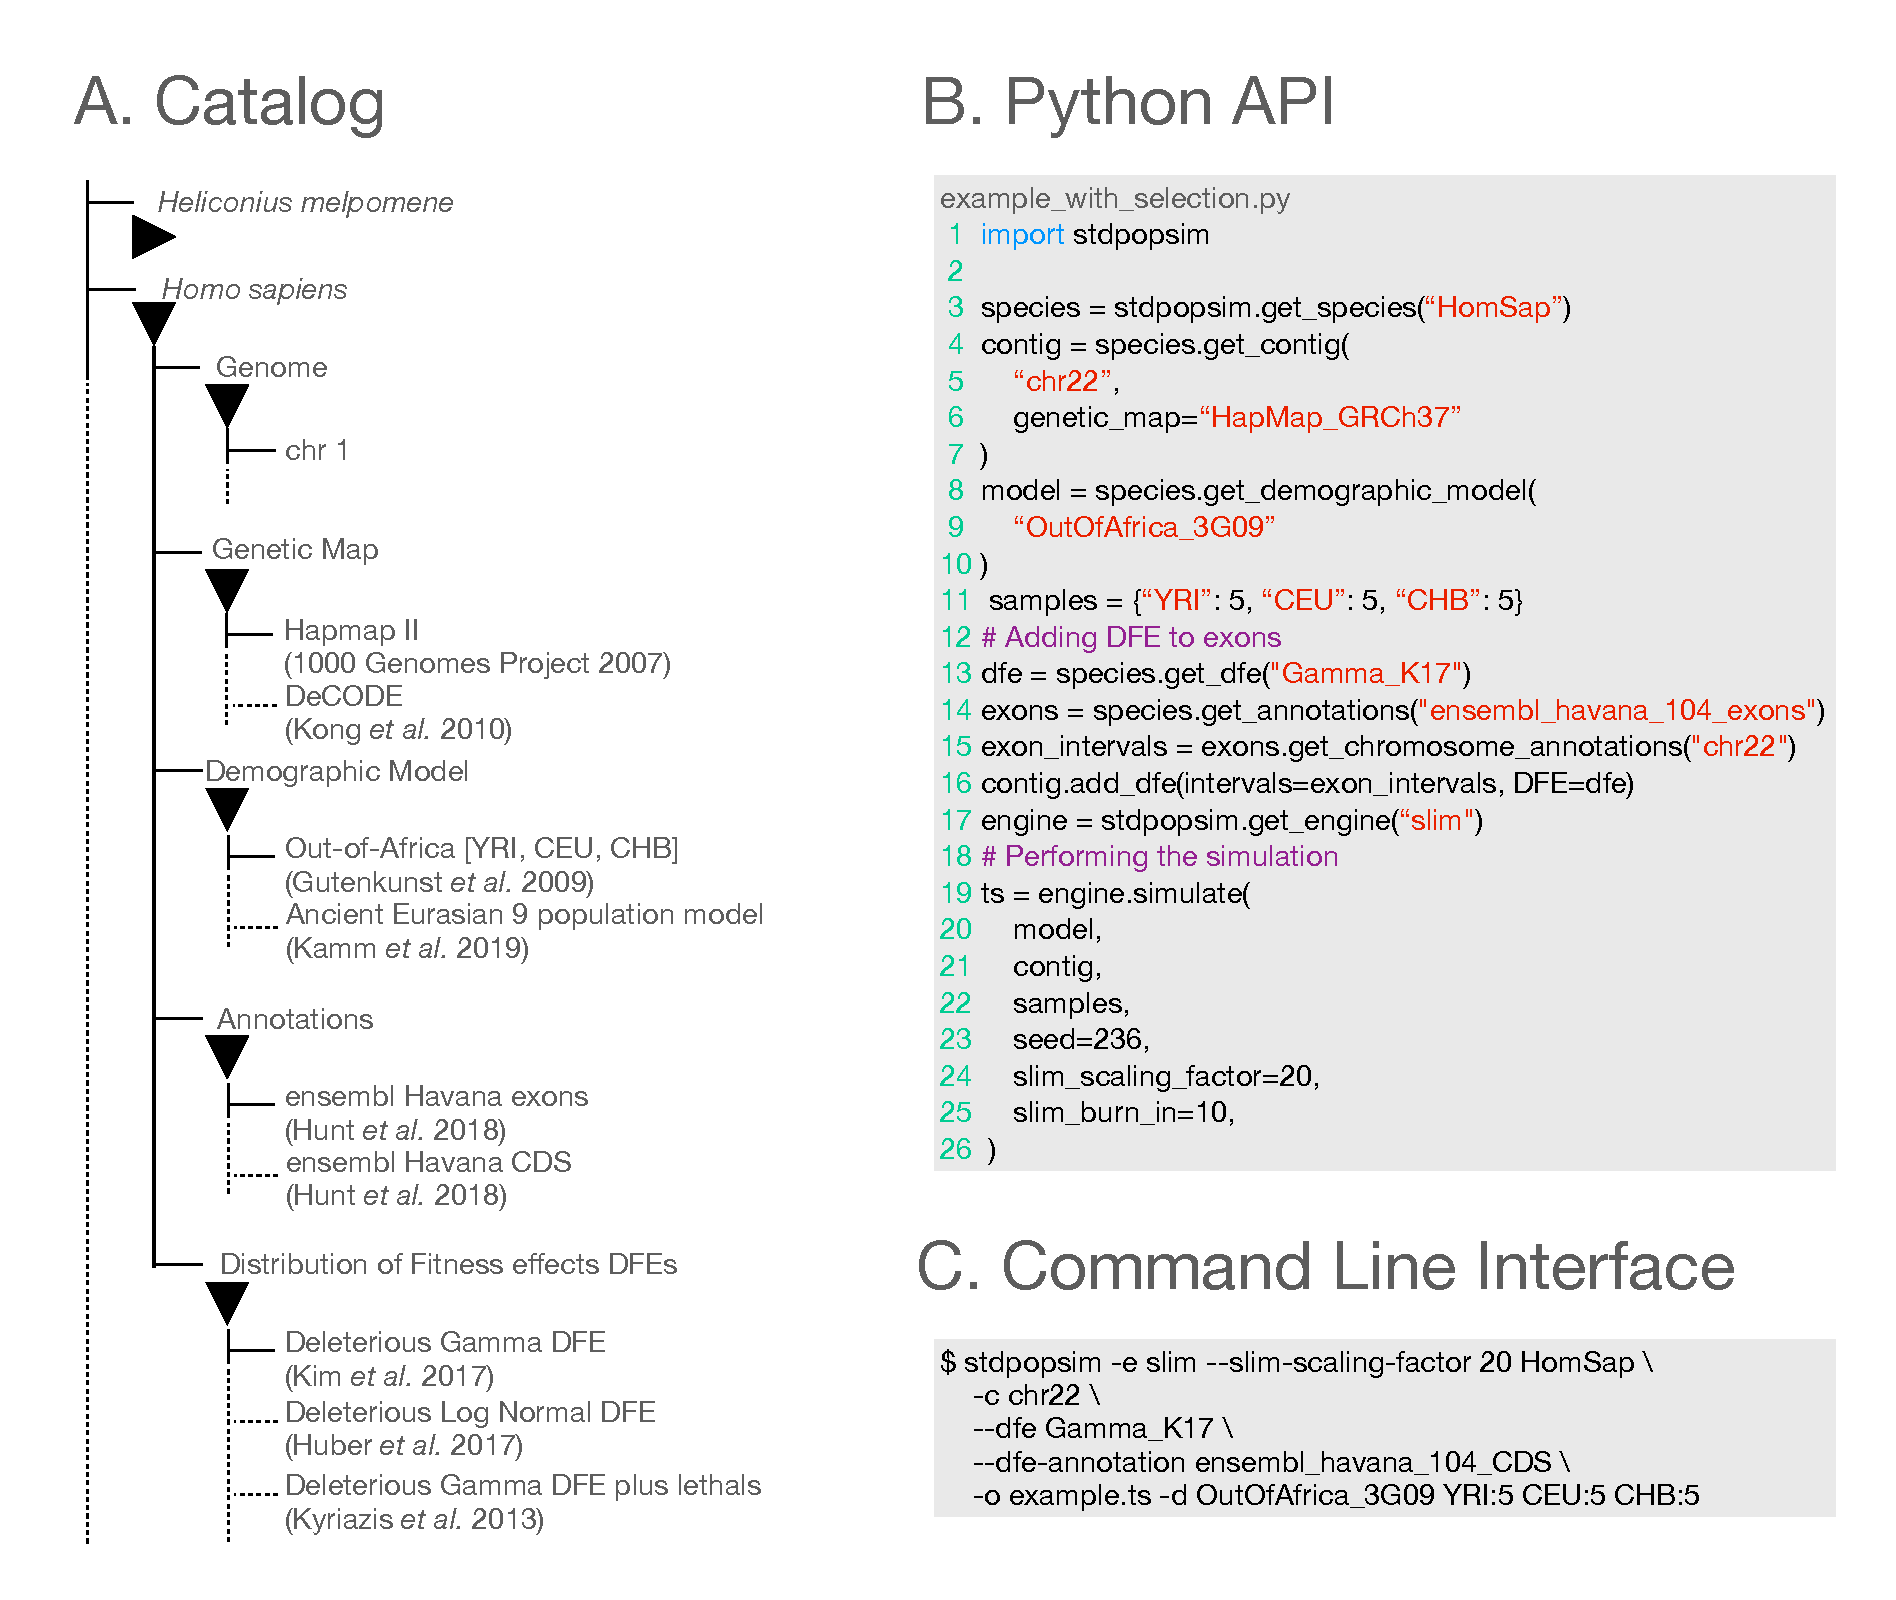
\includegraphics[width=\linewidth]{figures/schematics/catalog.pdf}
        \caption{\label{fig:schematic}
        A schematic of the \stdpopsim catalog for simulating genetic variation
        in a population. The user specifies a species, a portion of the genome to simulate,
        and optionally a genetic map, a model of demography, and a model of selection that 
        itself is composed of a distribution of fitness effects (DFE) and a set of functional
        annotations.}
    \end{wrapfigure}
\hfill
    
\section*{Example Applications with Selection}
In this section we provide a series of examples of how the new models of selection
in \stdpopsim can be used to benchmark and compare the performance of different
methods for inferring demographic history, selection, and the distribution of fitness
effects from genetic data. We focus on three main areas: demographic inference in the 
single and multi-population settings, inference of the distribution of fitness effects,
and the detection of selective sweeps, particularly in the context of background selection.

\section*{Inference of $N_e(t)$ in the context of selection}
One of the most common applications of population genetic inference is to estimate
the effective population size over time, $N_e(t)$, from genetic data. This can be done
using a variety of methods, including the pairwise sequentially Markovian coalescent
(PSMC) \citep{li2011inference}, through use of the site frequency spectrum (SFS),
as well as through identity by decent information. 
While that is so, it has been well described that selection, because of its effects on
local and more global patterns of genetic variation, can drive estimates of $N_e(t)$
further from true census population sizes simply because selection increases the 
rate of coalescence in the genome. 

Using \stdpopsim we can simulate genetic data under a model of selection and then 
examine the performance of different methods for inferring $N_e(t)$ from these simulated 
data. In Figure \ref{fig:1pop-human-demography} we show the results of such a benchmark
where we have simulated genomes under a model of human out of Africa (OOA) demography
with and without background selection on exons. For this simulation we have used
a genetic map from the 1000 Genomes Project along with a deleterious alleles DFE from \citep{huber2017determining}
that acts on exonic positions defined from the HAVANA group release 104 for the human genome. 
These simulations were then used to estimate $N_e(t)$ using four methods: 1) MSMC2 \citep{Schiffels2020}, 
2)the stairway plot method \citep{liu2020stairway}, 3) GONE \citep{santiago2020recent}, and 4) SMC++ \citep{terhorst2017robust}.

In Figure \ref{fig:1pop-human-demography} we show six panels, each of which shows the estimated $N_e(t)$
from each independent sample in a five-population model of human out-of-Africa demography
from Ragsdale \textit{et al.} (2019)
with samples taken from three modern geographic groups (CEU, CHB, and YRI from left to right).
The top row shows the results of simulations without background selection on exons, while the bottom row shows the results
of simulations with a Gamma distributed DFE on exons. In each panel we show the true $N_e(t)$ in black, and the estimated $N_e(t)$
in various colors for the four methods. Dotted lines on the bottom row are to visually reinforce that inference is done
from a model with selection.  We see that all methods perform reasonably in the absence of selection, 
although GONE seems to overestimate $N_e(t)$ in the more recent past for the CEU and CHB populations.
Presumably this could be due to patterns of linkage disequilibrium that result from the combination
of bottleneck and growth in these populations.
In the presence of selection, different methods behave differently. 
For instance stairwaiplot which uses the SFS to infer $N_e(t)$ seems to slightly underestimate $N_e(t)$
but is reasonably close to the true $N_e(t)$ in the absence of selection.
Likewise SMC++ seems to be more robust to the presence of selection,
but there is some added noise to the returned estimates. 
MSMC2 seems to be the most affected by the presence of selection, 
estimates of $N_e(t)$ varying quite a bit from the true $N_e(t)$.



\begin{figure}[t]
    \centering
    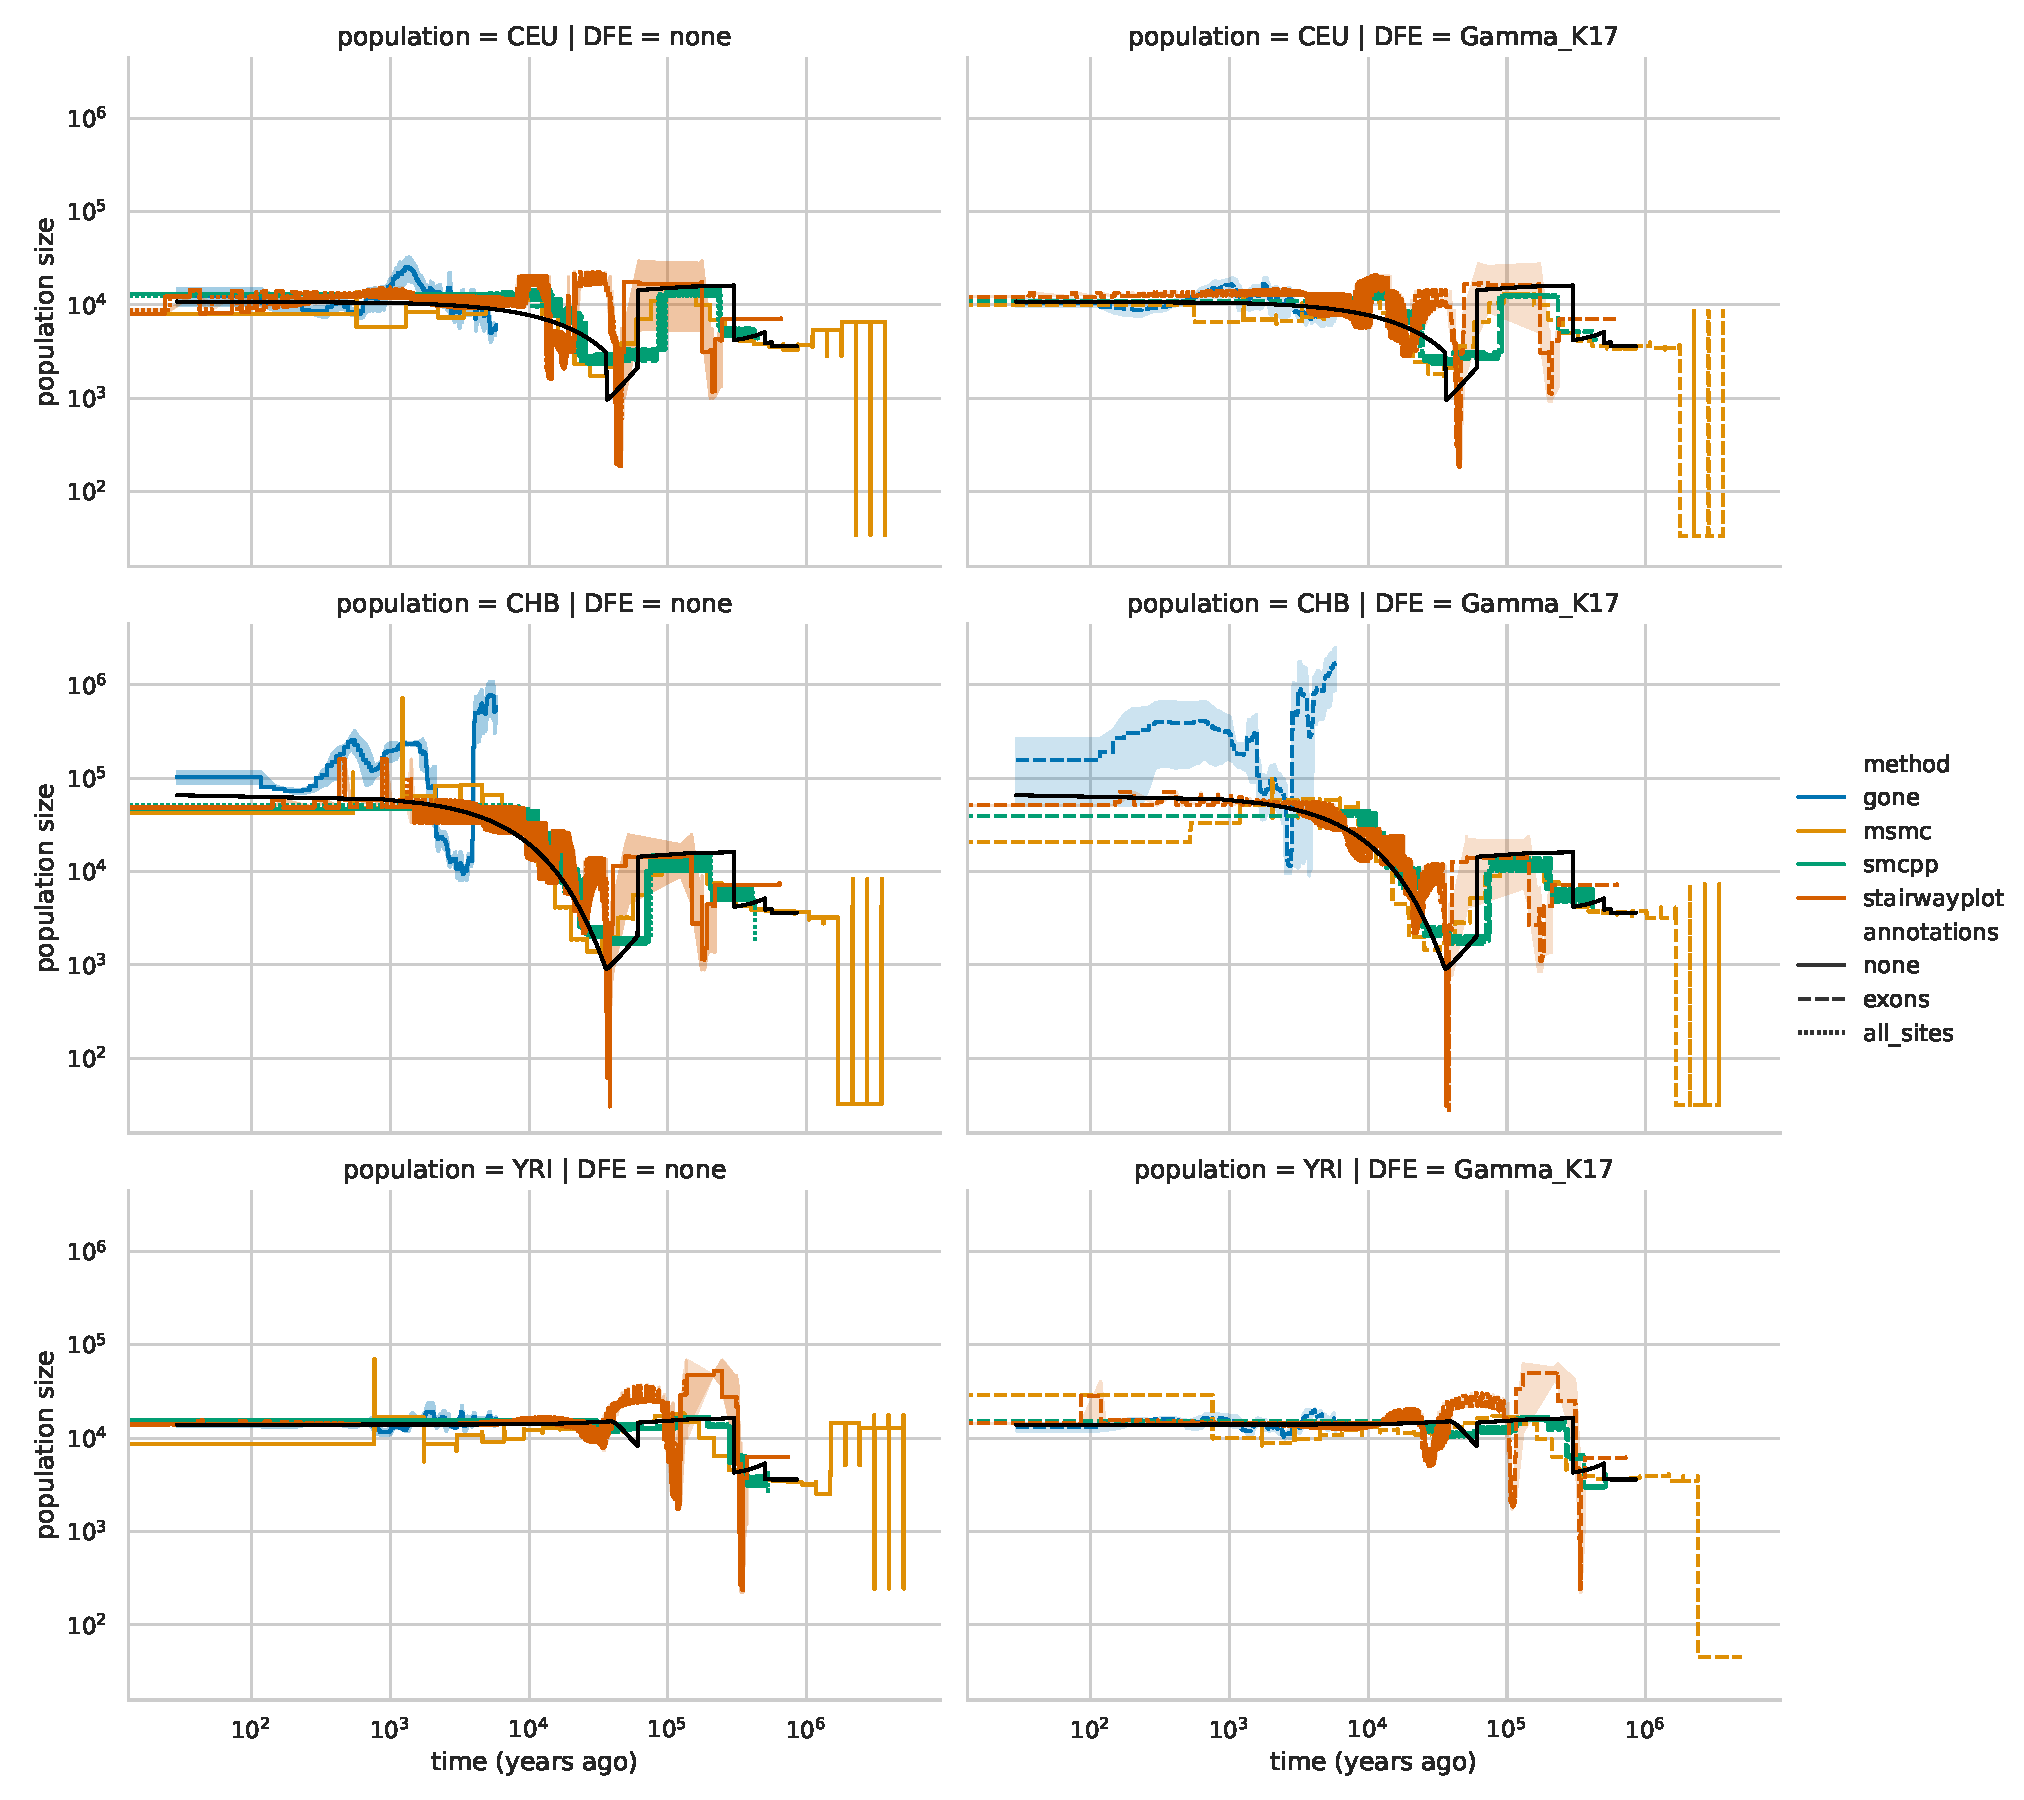
\includegraphics[width=\textwidth]{figures/HomSap/OOA/estimated_Ne_t_final}
    \caption{
    \label{fig:1pop-human-demography}
    Performance of methods to infer $N_e(t)$ from a human out-of-Africa model \citep{ragsdale2019models}
    with and without background selection on exons. The top row shows estimates of $N_e(t)$ from simulations
    without selection, while the bottom row shows estimates of $N_e(t)$ from simulations with a Gamma distributed   
    DFE acting on exons. In each panel we show the true $N_e(t)$ in black, and the estimated $N_e(t)$ from four methods:    
    MSMC2 \citep{Schiffels2020}, stairway plot \citep{liu2020stairway}, GONE \citep{santiago2020recent}, and SMC++ \citep{terhorst2017robust}.  
    }
\end{figure}

To highlight the ease of comparisons between different species and model enabled by \stdpopsim,
we have also performed a similar benchmark using the vaquita porpoise \textit{Phocoena sinus}.
In Figure \ref{fig:1pop-vaquita-demography} we show the results of $N_e(t)$ inference
where we have simulated genomes under a model of vaquita demography from \cite{robinson2022critically}.
For these simulations we have used the genome structure and exon annotations from the vaquita genome assembly
and a DFE from \cite{robinson2022critically} that acts on exonic positions, however no genetic map 
is currently available, so recombination rates are assumed to be constant across the genome.
The demographic model is a simple two-epoch model where population size has declined in the recent past
relative to the ancient past. 

In this case we see that all methods perform well both in the absence and presence of selection.


\begin{figure}[t]
    \centering
    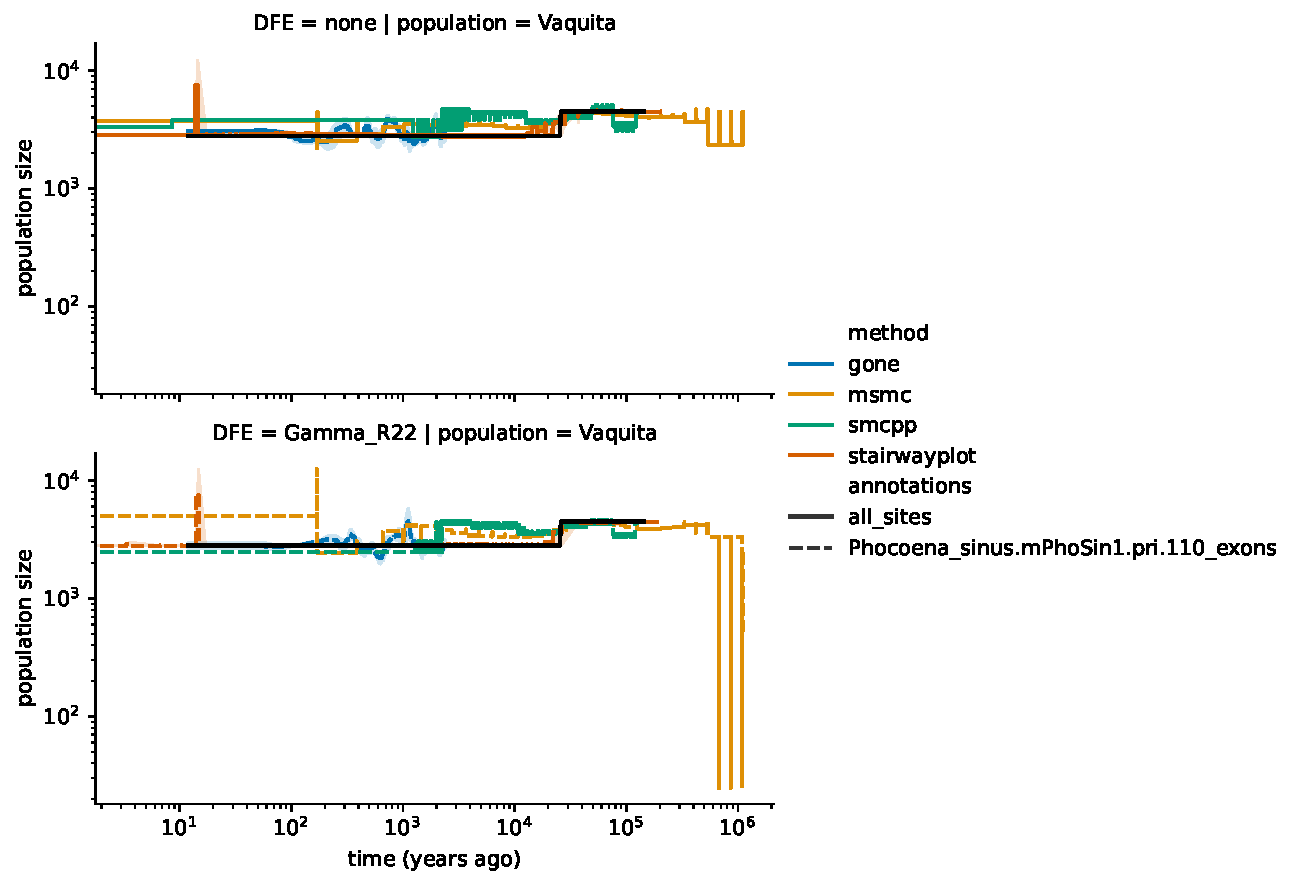
\includegraphics[width=\textwidth]{figures/PhoSin/Vaquita2Epoch_1R22/estimated_Ne_t_final}
    \caption{
    \label{fig:1pop-vaquita-demography}
    Performance of methods to infer $N_e(t)$ from a human out-of-Africa model \citep{ragsdale2019models}
    with and without background selection on exons. The top row shows estimates of $N_e(t)$ from simulations
    without selection, while the bottom row shows estimates of $N_e(t)$ from simulations with a Gamma distributed   
    DFE acting on exons. In each panel we show the true $N_e(t)$ in black, and the estimated $N_e(t)$ from four methods:    
    MSMC2 \citep{Schiffels2020}, stairway plot \citep{liu2020stairway}, GONE \citep{santiago2020recent}, and SMC++ \citep{terhorst2017robust}.  
    }
\end{figure}
\lipsum[20-25]

% \section*{outline}
%     \label{outline}
%     \begin{enumerate}
%         \item Single-population demographic inference methods
%         \begin{enumerate}
%             \item mscm2
%             \item stairwaiplot
%             \item GONE
%             \item SMC++
%         \end{enumerate}
%         \item Multi-population demographic inference methods
%         \begin{enumerate}
%             \item dadi
%             \item fastsimcoal
%             \item momi2
%         \end{enumerate}
%         \item DFE inference methods
%         \begin{enumerate}
%             \item dadi
%             \item polyDFE
%             \item DFE-alpha
%             \item GRAPES
%         \end{enumerate} 
%         \item sweeps
%         \begin{enumerate}
%             \item compare effect of BGS on sweep detection
%             \item compare power in different pops
%             \item compare methods
%         \end{enumerate}
%     \end{enumerate}

    




\section*{Example applications}
    \label{additions}



    \begin{figure}[ht]
        \centering
        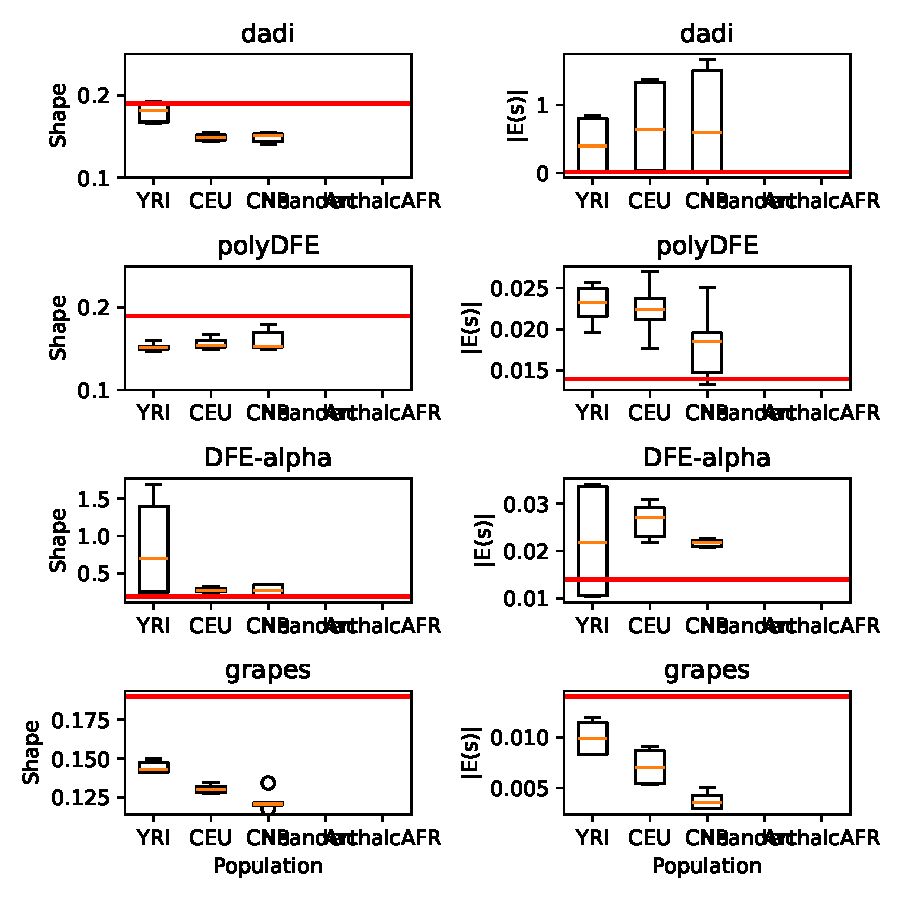
\includegraphics[width=\textwidth]{figures/HomSap/OOA/dfe.inference.benchmark}
        \caption{
        \label{fig:dfe_humans}
        Performance of methods to infer distribution of fitness effects (DFE).
        }
    \end{figure}


    % \begin{figure}[ht]
    %     \centering
    %     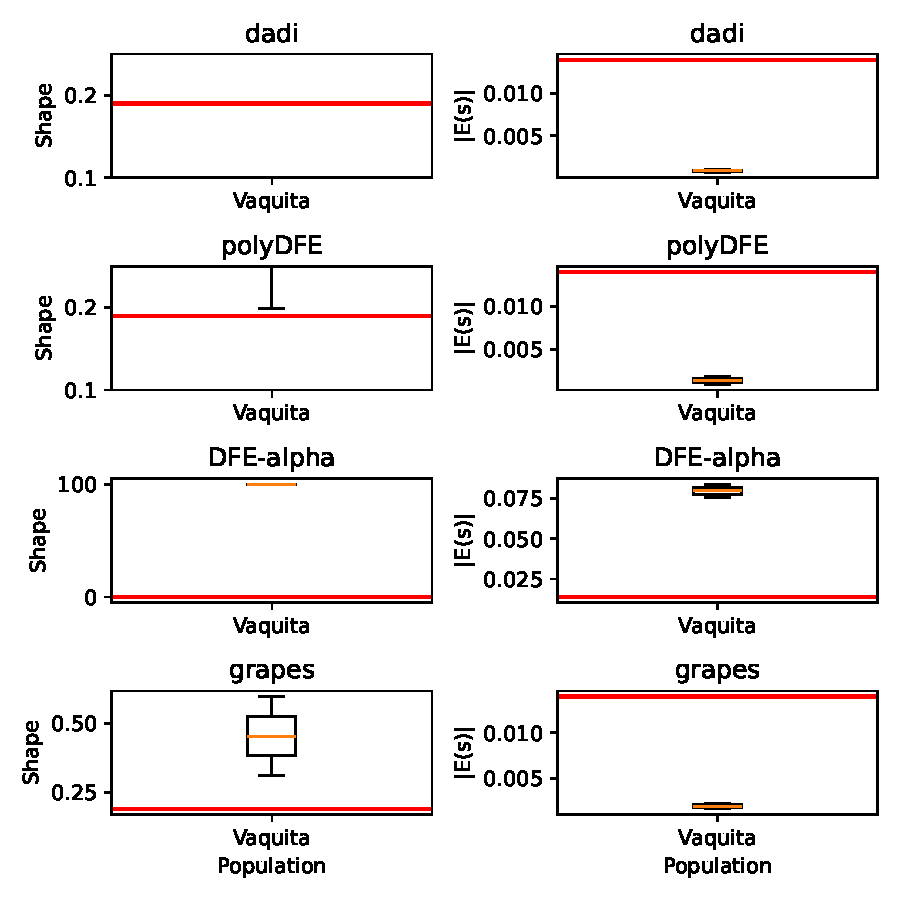
\includegraphics[width=\textwidth]{figures/PhoSin/dfe.inference.benchmark}
    %     \caption{
    %     \label{fig:dfe_vaquita}
    %     Performance of methods to infer distribution of fitness effects (DFE).
    %     }
    % \end{figure}


\section*{Conclusion}
    \label{conclusion}

\section*{Data availability}\label{data_availability}


\section*{Acknowledgments}\label{acknowledgements}

\section*{Funding}
    \label{funding}

\bibliography{references.bib}
\end{document}